\documentclass[11pt,a4paper]{article}
\usepackage[margin=18mm,top=22mm,bottom=20mm]{geometry}
\usepackage{fontspec}\setmainfont{Latin Modern Roman}
\usepackage{amsmath,amssymb,tikz,graphicx,fancyhdr,array,needspace}
\setlength{\headheight}{14pt}
\usetikzlibrary{arrows.meta}
\pagestyle{fancy}\fancyhf{}\renewcommand{\headrulewidth}{0.4pt}
\fancyhead[L]{\textbf{M-05}}\fancyhead[C]{\itshape Fizika (OliyFizika.uz mock test)}\fancyhead[R]{\textbf{Mock №5}}
\fancyfoot[C]{\thepage}
\setlength{\parindent}{0pt}\setlength{\parskip}{3pt}
\newcommand{\opt}[2]{\hspace*{4mm}#1)\ #2\par}
\newcommand{\blank}{\rule{5cm}{0.4pt}}
\begin{document}

\begin{center}{\Large\textbf{FIZIKA}}\end{center}
\noindent\begin{minipage}{\linewidth}
\textbf{1.}\ Uzunligi 1,5 m bölgan matematik mayatnik lift şiftiga osilgan. Lift pastga 4 m/s$^{2}$ tezlaniş bilan tuşayotgan bölsa, mayatnikning tebraniş davri (s) qanday? $g$=10 m/s$^{2}$\par\smallskip
\opt{A}{2,1}
\opt{B}{2,9}
\opt{C}{3,1}
\opt{D}{2,7}
\end{minipage}\vspace{9pt}\par
\noindent\begin{minipage}{\linewidth}
\textbf{2.}\ Muz ustida 80 kg massali odam 16 kg massali yukni sirpantirib yubordi. Yuk 4 s da 15 m masofa yurib töxtagan bölsa, odamning olgan eng katta kinetik energiyasini (J) hisoblang.\par\smallskip
\opt{A}{30}
\opt{B}{60}
\opt{C}{120}
\opt{D}{90}
\end{minipage}\vspace{9pt}\par
\noindent\begin{minipage}{\linewidth}
\textbf{3.}\ Bir jinsli $M$ massali sterjen rasmda körsatilganidek $m_1$=8 kg va $m_2$=6 kg massali yuklar bilan muvozanatga keltirilgan. $M$ massani (kg) aniqlang.\par\smallskip
\noindent\hspace*{4mm}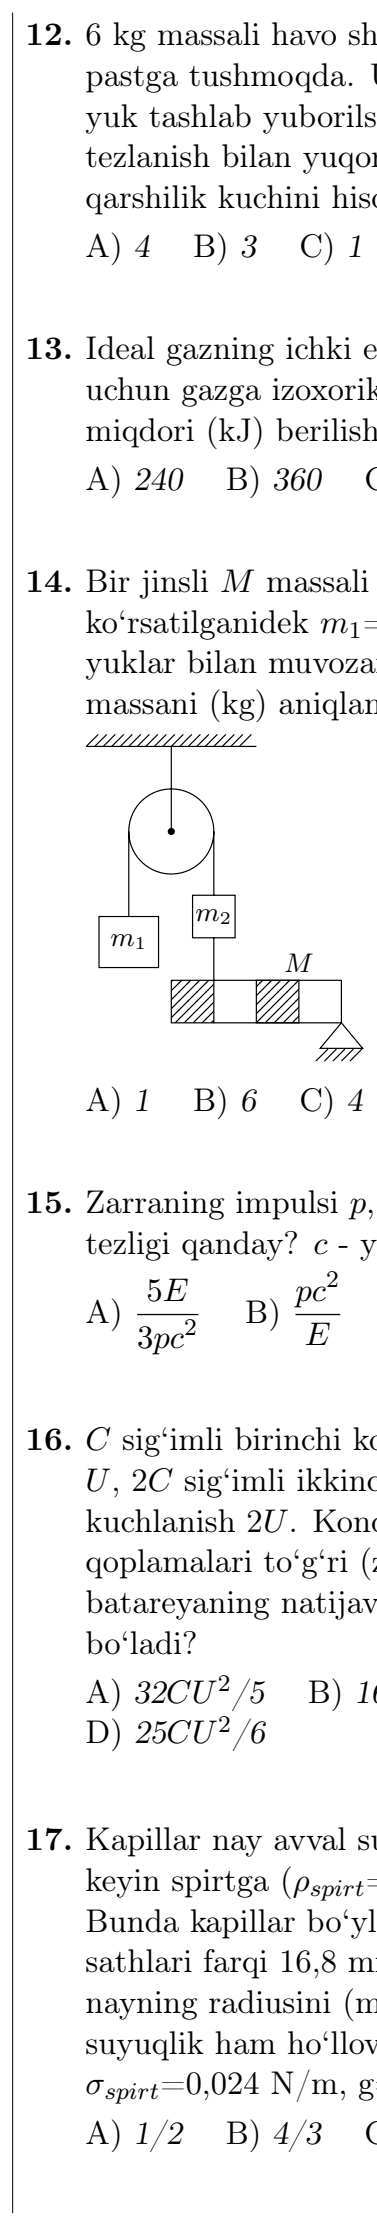
\includegraphics[width=0.6\linewidth,height=5.2cm,keepaspectratio]{../dtm-variantlari/rasmlar/1920945-14.png}\par\smallskip
\opt{A}{1}
\opt{B}{6}
\opt{C}{4}
\opt{D}{3}
\end{minipage}\vspace{9pt}\par
\noindent\begin{minipage}{\linewidth}
\textbf{4.}\ Jism 30 m/s boşlanğiç tezlik bilan tik yuqoriga otildi. Uning maksimal kötariliş balandligini (m) aniqlang.\par\smallskip
\opt{A}{30}
\opt{B}{45}
\opt{C}{90}
\opt{D}{15}
\end{minipage}\vspace{9pt}\par
\noindent\begin{minipage}{\linewidth}
\textbf{5.}\ Kosmik kema massasi 1220 kg bölib, tinç holatda turibdi. 80 kg massali kosmonavtni yengil qutqaruv zanjiri yordamida torta boşlaşdi. Agar kosmonavt va kosmik kema orasidagi boşlanğiç masofa 50 m ga teng bölsa, ular uçraşgunça kosmik kema qança masofani (m) ni ötadi?\par\smallskip
\opt{A}{3}
\opt{B}{47}
\opt{C}{25}
\opt{D}{50}
\end{minipage}\vspace{9pt}\par
\noindent\begin{minipage}{\linewidth}
\textbf{6.}\ $A$ nuqtadan boşlanğiç tezliksiz erkin taşlangan jism qiya tekislikka mutloq elastik urilib qaytdi va yerdagi $B$ nuqtaga kelib tuşdi. Agar jismning umumiy harakat vaqti 3 s bölsa, jismning köçiş modulini toping (m). g=10 m/s$^{2}$.\par\smallskip
\opt{A}{$5\sqrt{41}$}
\opt{B}{$\sqrt{41}$}
\opt{C}{$10\sqrt{41}$}
\opt{D}{5}
\end{minipage}\vspace{9pt}\par
\noindent\begin{minipage}{\linewidth}
\textbf{7.}\ 245 m balandlikda joylagan A nuqtadagi jism tik pastga erkin tuşişni boşlagan momentda B nuqtadagi manbadan tovuş tarqatildi. Agar tovuş 1 s ötgaç jismga yetib kelgan bölsa, tovuşning havoda tarqaliş tezligini aniqlang (m/s). g=10 m/s$^{2}$.\par\smallskip
\noindent\hspace*{4mm}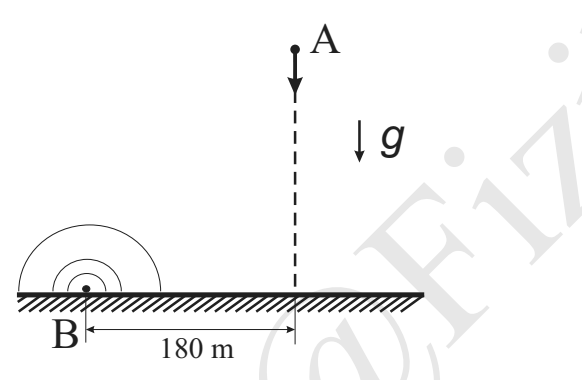
\includegraphics[width=0.6\linewidth,height=5.2cm,keepaspectratio]{../dtm-variantlari/rasmlar/T18-02.png}\par\smallskip
\opt{A}{320}
\opt{B}{300}
\opt{C}{333}
\opt{D}{340}
\end{minipage}\vspace{9pt}\par
\noindent\begin{minipage}{\linewidth}
\textbf{8.}\ Jism gorizontga nisbatan qiyalatib $E$ kinetik energiya bilan otildi. Trayektoriyasining eng yuqori nuqtasida jismning kinetik energiyasi $E/4$ ga kamaygan bölsa, jism qanday burçak ($^\circ$) ostida otilganini aniqlang.\par\smallskip
\opt{A}{30}
\opt{B}{60}
\opt{C}{37}
\opt{D}{45}
\end{minipage}\vspace{9pt}\par
\noindent\begin{minipage}{\linewidth}
\textbf{9.}\ Muhitda tezligi 4 m/s, tölqin uzunligi 4$\pi$ m bölgan köndalang tölqin hosil qilinmoqda. Agar muhit zarralarining maksimal tezligi 20 cm/s bölsa, tebraniş amplitudasini (cm) aniqlang.\par\smallskip
\opt{A}{5}
\opt{B}{10}
\opt{C}{20}
\opt{D}{15}
\end{minipage}\vspace{9pt}\par
\noindent\begin{minipage}{\linewidth}
\textbf{10.}\ Örtaça tezligi 20 m/s bölgan jism 6 s da qança masofa (m) bosadi?\par\smallskip
\opt{A}{60}
\opt{B}{20}
\opt{C}{120}
\opt{D}{40}
\end{minipage}\vspace{9pt}\par
\noindent\begin{minipage}{\linewidth}
\textbf{11.}\ Biror ideal gazning özgarmas hajmdagi molyar issiqlik siğimi CV va özgarmas bosimdagi molyar issiqlik siğimi CP bölsa, javoblardan töğrisini toping.\par\smallskip
\opt{A}{1 atomli gazlar uçun CV = 3R/2}
\opt{B}{2 atomli gazlar uçun CV = 3R}
\opt{C}{3 atomli gazlar uçun CP = 7R/2}
\opt{D}{2 atomli gazlar uçun CP = 4R}
\end{minipage}\vspace{9pt}\par
\noindent\begin{minipage}{\linewidth}
\textbf{12.}\ Ideal gaz (bir atomli) grafikda körsatilganidek 1-2 jarayonda 2,5 kJ issiqlik miqdori berib qizdirildi, 2-3 jarayonda 3 kJ issiqlik miqdori olib sovitildi. Bu ikki jarayonda gazning içki energiyasi (kJ) qançaga özgardi?\par\smallskip
\noindent\hspace*{4mm}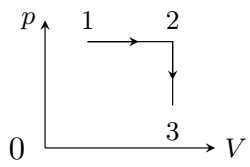
\includegraphics[width=0.6\linewidth,height=5.2cm,keepaspectratio]{../dtm-variantlari/rasmlar/8000009-29.png}\par\smallskip
\opt{A}{1,2}
\opt{B}{0,5}
\opt{C}{2}
\opt{D}{1,5}
\end{minipage}\vspace{9pt}\par
\noindent\begin{minipage}{\linewidth}
\textbf{13.}\ Havo harorati $t_1$=24 $^\circ$C, nisbiy namlik 95 \%. Agar harorat $t_2$=16 $^\circ$C bölib qolgan bölsa, havoning 1 m$^{3}$ hajmidan neça gramm şudring tuşadi? $t_1$=24 $^\circ$C va $t_2$=16 $^\circ$C haroratlardagi töyingan buğ bosimlari mos ravişda 21,8 g/m$^{3}$ va 13,6 g/m$^{3}$.\par\smallskip
\opt{A}{7,11}
\opt{B}{8,93}
\opt{C}{11,1}
\opt{D}{4,78}
\end{minipage}\vspace{9pt}\par
\noindent\begin{minipage}{\linewidth}
\textbf{14.}\ 20 $^\circ$C da töyingan simob buğining ziçligi 0,02 g/m$^{3}$ ga teng. Şu temperaturada buğ bosimini toping (Pa). M=208 g/mol.\par\smallskip
\opt{A}{0,6}
\opt{B}{0,9}
\opt{C}{0,24}
\opt{D}{24}
\end{minipage}\vspace{9pt}\par
\noindent\begin{minipage}{\linewidth}
\textbf{15.}\ Normal şaroitda har qanday ideal gazning 1 m$^{3}$ hajmida qança molekula mavjud?\par\smallskip
\opt{A}{2,7$\cdot10^{24}$}
\opt{B}{2,24$\cdot10^{25}$}
\opt{C}{2,7$\cdot10^{25}$}
\opt{D}{6,02$\cdot10^{23}$.}
\end{minipage}\vspace{9pt}\par
\noindent\begin{minipage}{\linewidth}
\textbf{16.}\ 4 ta bir xil batareya qutblari qarama-qarşi qilib ketma-ket ulangan. Agar tizimning umumiy kuçlanişi 8 V ga teng bölsa, bitta batareyaning kuçlanişini (V) aniqlang.\par\smallskip
\opt{A}{4}
\opt{B}{8}
\opt{C}{2}
\opt{D}{1}
\end{minipage}\vspace{9pt}\par
\noindent\begin{minipage}{\linewidth}
\textbf{17.}\ Zanjirning bir qismi ketma-ket ulangan pölat ($S_1$=0,48 mm$^{2}$, $l_1$=2 m) va nikelin ($S_2$=0,21 mm$^{2}$, $l_2$=1 m) simlardan tuzilgan. 0,6 A tok kuçini hosil qiliş uçun mazkur qismga qanday kuçlaniş qöyilişi lozim (V)? Pölat va nikelin simlarning soliştirma qarşiliklari mos ravişda $12\cdot10^{-8}$ $\Omega\cdot$m va $42\cdot10^{-8}$ $\Omega\cdot$m.\par\smallskip
\opt{A}{1,5}
\opt{B}{1}
\opt{C}{2}
\opt{D}{1,8}
\end{minipage}\vspace{9pt}\par
\noindent\begin{minipage}{\linewidth}
\textbf{18.}\ Içki qarşiligi 40 m$\Omega$ bölgan tok manbai qisqa tutaşganda, tok kuçi 300 A böldi. Manbaning EYK ini aniqlang (V).\par\smallskip
\opt{A}{9}
\opt{B}{10}
\opt{C}{12}
\opt{D}{24}
\end{minipage}\vspace{9pt}\par
\noindent\begin{minipage}{\linewidth}
\textbf{19.}\ Birinçi tökli xalqa gorizontal sirtda yotibti. Uning yoniga ikkinçi tökli xalqa rasmda körsatilganidek joylaştirilsa birinçi xalqa markazidagi magnit maydon induksiyasi qanday özgaradi?\par\smallskip
\noindent\hspace*{4mm}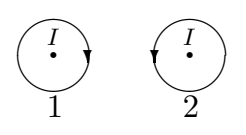
\includegraphics[width=0.6\linewidth,height=5.2cm,keepaspectratio]{../dtm-variantlari/rasmlar/8000537-22.png}\par\smallskip
\opt{A}{ortadi}
\opt{B}{5 marta kamayadi}
\opt{C}{2 marta kamayadi}
\opt{D}{özgarmaydi}
\end{minipage}\vspace{9pt}\par
\noindent\begin{minipage}{\linewidth}
\textbf{20.}\ Radiusi 1 mm bölgan silindrik mis sim orqali 3,14 A tok ötmoqda. Tok ziçligini aniqlang (A/m$^{2}$).\par\smallskip
\opt{A}{$2\cdot10^5$}
\opt{B}{$6{,}28\cdot10^5$}
\opt{C}{$1\cdot10^6$}
\opt{D}{$3{,}14\cdot10^6$}
\end{minipage}\vspace{9pt}\par
\noindent\begin{minipage}{\linewidth}
\textbf{21.}\ Öramlar soni 200 ta bölgan ğaltakdan 2 A özgarmas tok ötmoqda. Agar ğaltak özagining magnit kiruvçanligi 100 ga teng bölsa, uning magnit maydon induksiyasini hisoblang (mT). Ğaltak uzunligi 10 cm.\par\smallskip
\opt{A}{150$\pi$}
\opt{B}{100$\pi$}
\opt{C}{16$\pi$}
\opt{D}{160$\pi$}
\end{minipage}\vspace{9pt}\par
\noindent\begin{minipage}{\linewidth}
\textbf{22.}\ Mis simning 0 $^\circ$C temperaturadagi qarşiligi 50 $\Omega$ ga, 30 $^\circ$C temperaturadagi qarşiligi esa 57,5 $\Omega$ ga teng böldi. Uning termik koeffitsiyentini (10$^{-3}$ K$^{-1}$) aniqlang.\par\smallskip
\opt{A}{2}
\opt{B}{4}
\opt{C}{5}
\opt{D}{6}
\end{minipage}\vspace{9pt}\par
\noindent\begin{minipage}{\linewidth}
\textbf{23.}\ Quyidagi fikrlarning qaysilari töğri? 1) teskari $p-n$ ötişda yarim ötkazgiçli diodning berkituvçi qatlami kengayadi; 2) metallarda elektr toki manfiy ionlarning tartibli harakatidan iborat; 3) diod bu - bitta $p-n$ ötişga ega bölgan yarimötkazgiçli asbob; 4) $p$ turdagi yarimötkazgiçlarda asosiy zaryad taşuvçilar – elektronlar\par\smallskip
\opt{A}{2, 4}
\opt{B}{1, 4}
\opt{C}{1, 3}
\opt{D}{1, 2}
\end{minipage}\vspace{9pt}\par
\noindent\begin{minipage}{\linewidth}
\textbf{24.}\ Rasmdagi sxemada AB qismlar orasidagi umumiy elektr siğimni hisoblang.\par\smallskip
\noindent\hspace*{4mm}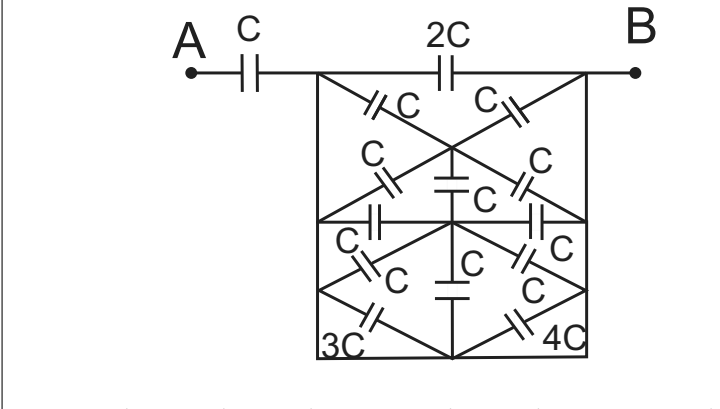
\includegraphics[width=0.6\linewidth,height=5.2cm,keepaspectratio]{../dtm-variantlari/rasmlar/T09-27.png}\par\smallskip
\opt{A}{4C/3}
\opt{B}{101C/3}
\opt{C}{0,5C}
\opt{D}{C}
\end{minipage}\vspace{9pt}\par
\noindent\begin{minipage}{\linewidth}
\textbf{25.}\ Özgaruvçan tok zanjirida reaktiv qarşilik $4\ \Omega$, aktiv qarşilik $5\ \Omega$, özgaruvçan tok amplitudasi $2\sqrt2$ A. Tokning örtaça quvvati (W) topilsin.\par\smallskip
\opt{A}{12,5}
\opt{B}{40}
\opt{C}{39}
\opt{D}{20}
\end{minipage}\vspace{9pt}\par
\noindent\begin{minipage}{\linewidth}
\textbf{26.}\ Nuqta fokus masofasi 20 cm bölgan yupqa yiğuvçi linzaning boş optik öqidan 1 cm balandlikda turibdi. Nuqta va linza orasidagi masofa 25 cm. Uning tasviri bu öqdan qanday masofada (cm) hosil bölgan?\par\smallskip
\opt{A}{1}
\opt{B}{2}
\opt{C}{4}
\opt{D}{3}
\end{minipage}\vspace{9pt}\par
\noindent\begin{minipage}{\linewidth}
\textbf{27.}\ Optik kuçi 2 dptr bölgan linzaning fokus masofasini (m) aniqlang.\par\smallskip
\opt{A}{2}
\opt{B}{0,5}
\opt{C}{1}
\opt{D}{0,2}
\end{minipage}\vspace{9pt}\par
\noindent\begin{minipage}{\linewidth}
\textbf{28.}\ Suv töldirilgan hovuzga vertikal yuqoridan qaralganda çuqurligi 6 m körinsa, uning haqiqiy çuqurligi qançaga (m) teng?\par\smallskip
\opt{A}{6}
\opt{B}{10}
\opt{C}{8}
\opt{D}{4,8}
\end{minipage}\vspace{9pt}\par
\noindent\begin{minipage}{\linewidth}
\textbf{29.}\ Ma’lumki, ikkita proton bir-biridan kulon kuçi vositasida itarişişadi. Qanday holatda ular bir-biriga tortiladi?\par\smallskip
\opt{A}{özaro teskari parallel yönalişda öta katta tezlikda harakatlanganda}
\opt{B}{özaro bir xil yönalişda parallel öta katta tezlikda harakatlanganda}
\opt{C}{özaro teskari yönalişda öta katta tezlikda bir-biridan uzoqlaşsa}
\opt{D}{heç qaçon ular tortişmaydilar}
\end{minipage}\vspace{9pt}\par
\noindent\begin{minipage}{\linewidth}
\textbf{30.}\ Sindiriş körsatkiçi 1,5 bölgan şaffof muhitda çastotasi 6$\cdot10^{14}$ Hz bölgan foton tarqalmoqda. Fotonning impulsini (kg$\cdot$m/s) toping. Plank doimiysi 6,62$\cdot10^{-34}$ J$\cdot$s ga teng.\par\smallskip
\opt{A}{1,32$\cdot10^{-30}$}
\opt{B}{1,99$\cdot10^{-27}$}
\opt{C}{1,32$\cdot10^{-29}$}
\opt{D}{1,99$\cdot10^{-29}$}
\end{minipage}\vspace{9pt}\par
\noindent\begin{minipage}{\linewidth}
\textbf{31.}\ Birinçi zarra tezligi 0,95$c$ bölgan ikkinçi zarraga yetib olmoqda. Ularning nisbiy tezligi 0,2$c$ bölsa, birinçi zarraning tezligi qanday? ($c$-yoruğlikning vakuumdagi tezligi)\par\smallskip
\opt{A}{0,99$c$}
\opt{B}{0,97$c$}
\opt{C}{0,9$c$}
\opt{D}{1,15$c$}
\end{minipage}\vspace{9pt}\par
\noindent\begin{minipage}{\linewidth}
\textbf{32.}\ Mutloq qora sirtning bir kvadrat santimetrli yuzasi har sekundda tölqin uzunligi 400 nm bölgan 2,8$\cdot10^{17}$ ta kvant yutmoqda. Nurning bosimi ($\mu$Pa) qanday? h=6,63$\cdot10^{-34}$ J$\cdot$s.\par\smallskip
\opt{A}{2,3}
\opt{B}{4,6}
\opt{C}{460}
\opt{D}{540}
\end{minipage}\vspace{9pt}\par
\newpage\noindent\textbf{33–35-test topshiriqlariga mos keluvchi javoblarni (A–F) javob variantlaridan tanlang.}\par\smallskip
Rasmda elektr zanjir tasvirlangan. Batareyaning ichki qarshiligi nolga teng, ampermetrlar ideal.\par\medskip
\begin{center}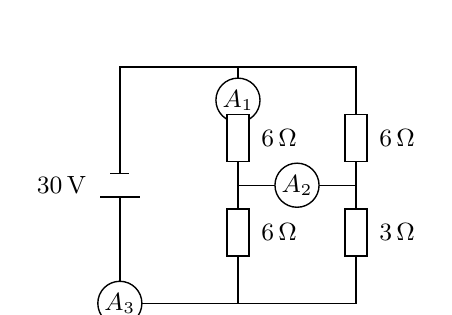
\begin{tikzpicture}[line width=0.5pt]
\draw (0,0)--(0,1.35); \draw (0,1.65)--(0,3)--(3,3)--(3,2.4); \draw (-0.25,1.35)--(0.25,1.35); \draw (-0.12,1.65)--(0.12,1.65);
\node[left] at (-0.3,1.5) {\small $30\,\mathrm{V}$};
\draw (1.5,3)--(1.5,2.72); \draw (1.5,2.44)--(1.5,2.4);
\draw (1.5,1.8)--(1.5,1.2); \draw (1.5,0.6)--(1.5,0)--(0.28,0); \draw (-0.28,0)--(0,0);
\draw (3,1.8)--(3,1.2); \draw (3,0.6)--(3,0)--(1.5,0);
\draw (1.5,1.5)--(1.97,1.5); \draw (2.53,1.5)--(3,1.5);
\draw[fill=white] (1.5,2.58) circle (0.28); \node at (1.5,2.58) {\small $A_1$};
\draw[fill=white] (1.3599999999999999,1.8) rectangle (1.6400000000000001,2.4); \node[right] at (1.67,2.1) {\small $6\,\Omega$};
\draw[fill=white] (1.3599999999999999,0.6000000000000001) rectangle (1.6400000000000001,1.2); \node[right] at (1.67,0.9) {\small $6\,\Omega$};
\draw[fill=white] (2.86,1.8) rectangle (3.14,2.4); \node[right] at (3.17,2.1) {\small $6\,\Omega$};
\draw[fill=white] (2.86,0.6000000000000001) rectangle (3.14,1.2); \node[right] at (3.17,0.9) {\small $3\,\Omega$};
\draw[fill=white] (2.25,1.5) circle (0.28); \node at (2.25,1.5) {\small $A_2$};
\draw[fill=white] (0.0,0.0) circle (0.28); \node at (0.0,0.0) {\small $A_3$};
\end{tikzpicture}\end{center}
\noindent\fbox{\begin{minipage}{0.64\linewidth}\vspace{4pt}\textbf{33.}\ $A_1$ ampermetrning körsatişini (A) aniqlang.\\[6pt]\textbf{34.}\ $A_2$ ampermetrning körsatişini (A) aniqlang.\\[6pt]\textbf{35.}\ $A_3$ ampermetrning körsatişini (A) aniqlang.\vspace{4pt}\end{minipage}\vrule\hspace{6pt}\begin{minipage}{0.28\linewidth}\vspace{4pt}A)\ 3\\B)\ 6\\C)\ 5\\D)\ 1\\E)\ 2\\F)\ 1,5\vspace{4pt}\end{minipage}}\par\vspace{14pt}
\Needspace{9\baselineskip}
\noindent\textbf{36.}\ Qirrasining uzunligi 5 cm bölgan kub şaklidagi 1 ta muz bölagi asosining yuzasi 150 cm$^2$ bölgan, 112,5 g suv quyilgan silindrik idişda taşlandi. $\rho_{muz}=900$ kg/m$^3$.\par\smallskip
\medskip\noindent\textbf{a)\ Muzlar erib ketgandan söng suyuqlikning idiş tubiga beradigan bosimini (Pa) toping.}\par
\noindent\textit{Javob}: a)\ \blank\par
\medskip\noindent\textbf{b)\ Muzlar erib ketgandan söng suyuqlikning idiş tubiga beradigan bosim kuçini (N) hisoblang.}\par
\noindent\textit{Javob}: b)\ \blank\par
\medskip\noindent\textbf{Diqqat!} Javoblaringizni javoblar varaqasiga köçirib yozing.\par\vspace{10pt}
\Needspace{9\baselineskip}
\noindent\textbf{37.}\ Silindrik idişga teng massali suv va kerosin quyildi. Suyuqliklar ustunining umumiy balandligi 27 cm ga teng. $\rho_{kerosin}=800$ kg/m$^3$.\par\smallskip
\medskip\noindent\textbf{a)\ Suv ustunining balandligini (cm) aniqlang.}\par
\noindent\textit{Javob}: a)\ \blank\par
\medskip\noindent\textbf{b)\ Idiş tubidan 5 cm balandlikdagi nuqtada suyuqliklarning hosil qilgan umumiy bosimini (Pa) toping.}\par
\noindent\textit{Javob}: b)\ \blank\par
\medskip\noindent\textbf{Diqqat!} Javoblaringizni javoblar varaqasiga köçirib yozing.\par\vspace{10pt}
\Needspace{9\baselineskip}
\noindent\textbf{38.}\ Uzunligi 27 m, qiyalik burçagi $37^\circ$ bölgan silliq qiya tekislik tepasidan 8 kg massali jism sirpanib tuşdi. $\sin37^\circ=0,6$, $\cos37^\circ=0,8$.\par\smallskip
\medskip\noindent\textbf{a)\ Jismning qiya tekislik etagidagi tezligini (m/s) toping.}\par
\noindent\textit{Javob}: a)\ \blank\par
\medskip\noindent\textbf{b)\ Bu jarayonda oğirlik kuçining bajargan işini (J) toping.}\par
\noindent\textit{Javob}: b)\ \blank\par
\medskip\noindent\textbf{Diqqat!} Javoblaringizni javoblar varaqasiga köçirib yozing.\par\vspace{10pt}
\Needspace{9\baselineskip}
\noindent\textbf{39.}\ Bir atomli ideal gazga 200 J issiqlik berib, hajmi izobarik ravişda 3 marta oşirildi.\par\smallskip
\medskip\noindent\textbf{a)\ Bunda gazning absolyut temperaturasi qanday özgaradi?}\par
\noindent\textit{Javob}: a)\ \blank\par
\medskip\noindent\textbf{b)\ Gazning bajargan işini (J) aniqlang.}\par
\noindent\textit{Javob}: b)\ \blank\par
\medskip\noindent\textbf{Diqqat!} Javoblaringizni javoblar varaqasiga köçirib yozing.\par\vspace{10pt}
\Needspace{9\baselineskip}
\noindent\textbf{40.}\ Issiqlik siğimi 250 J/K bölgan idişda 12 $^\circ$C temperaturali 2 $\ell$ suv bor. Idişga $-6\,^\circ$C temperaturali 1 kg muz taşlandi. $c_{suv}=4200$ J/(kg$\cdot$K), $c_{muz}=2100$ J/(kg$\cdot$K), $\lambda_{muz}=330$ kJ/kg.\par\smallskip
\medskip\noindent\textbf{a)\ Natijaviy temperaturani ($^\circ$C) toping.}\par
\noindent\textit{Javob}: a)\ \blank\par
\medskip\noindent\textbf{b)\ Muzning olgan issiqlik miqdorini (kJ) aniqlang.}\par
\noindent\textit{Javob}: b)\ \blank\par
\medskip\noindent\textbf{Diqqat!} Javoblaringizni javoblar varaqasiga köçirib yozing.\par\vspace{10pt}
\Needspace{9\baselineskip}
\noindent\textbf{41.}\ Proton induksiyasi $B$ bölgan magnit maydonga tik uçib kirdi va $r$ radiusli aylana böylab harakatlana boşladi. $m$ — zarraning massasi, $e$ — elementar zaryad.\par\smallskip
\medskip\noindent\textbf{a)\ Uning kinetik energiyasini aniqlang.}\par
\noindent\textit{Javob}: a)\ \blank\par
\medskip\noindent\textbf{b)\ Unga ta’sir etayotgan Lorens kuçini aniqlang.}\par
\noindent\textit{Javob}: b)\ \blank\par
\medskip\noindent\textbf{Diqqat!} Javoblaringizni javoblar varaqasiga köçirib yozing.\par\vspace{10pt}
\Needspace{9\baselineskip}
\noindent\textbf{42.}\ Maydon kuçlanganligi $E$ bölgan bir jinsli elektr maydonda harakatlanayotgan proton $l$ masofaga köçib, $A$ nuqtadan $B$ nuqtaga yetib bordi (rasmda $AD\perp \vec E$).\par\smallskip
\begin{center}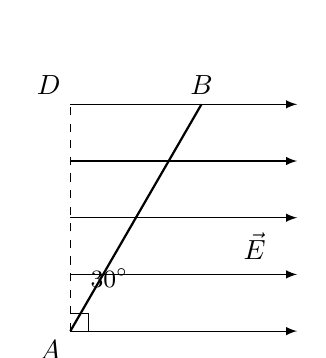
\begin{tikzpicture}[scale=0.9]\foreach \y in {0,0.8,1.6,2.4,3.2}{\draw[-latex] (0,\y)--(3.2,\y);}\draw (0.25,0)--(0.25,0.25)--(0,0.25);\draw[dashed] (0,0)--(0,3.2);\draw[thick] (0,0)--(1.85,3.2);\node[below left] at (0,0) {$A$};\node[above left] at (0,3.2) {$D$};\node[above] at (1.85,3.2) {$B$};\node at (2.6,1.2) {$\vec E$};\node at (0.55,0.75) {\small $30^\circ$};\end{tikzpicture}\end{center}
\medskip\noindent\textbf{a)\ Zarraning kinetik energiyasi qançaga özgarganini aniqlang.}\par
\noindent\textit{Javob}: a)\ \blank\par
\medskip\noindent\textbf{b)\ Zarra $ABDA$ yopiq yöl böylab köçirilganda elektr kuçlar bajaradigan işni aniqlang.}\par
\noindent\textit{Javob}: b)\ \blank\par
\medskip\noindent\textbf{Diqqat!} Javoblaringizni javoblar varaqasiga köçirib yozing.\par\vspace{10pt}
\Needspace{9\baselineskip}
\noindent\textbf{43.}\ Şişadagi nurning intensivligi 60 W/m$^2$ ga teng. $c=3\cdot10^8$ m/s.\par\smallskip
\medskip\noindent\textbf{a)\ Nurdagi elektromagnit maydon energiyasining ziçligini (J/m$^3$) aniqlang.}\par
\noindent\textit{Javob}: a)\ \blank\par
\medskip\noindent\textbf{b)\ Nur şişadagi közgudan tik akslansa, közguga beradigan bosimini (Pa) aniqlang.}\par
\noindent\textit{Javob}: b)\ \blank\par
\medskip\noindent\textbf{Diqqat!} Javoblaringizni javoblar varaqasiga köçirib yozing.\par\vspace{10pt}
\Needspace{9\baselineskip}
\noindent\textbf{44.}\ Oyning diametri $3,5\cdot10^{6}$ m ga, Yer bilan Oyn orasidagi masofa $3,8\cdot10^{8}$ m ga teng. Fokus masofasi 1 m bölgan Yerdagi linza ekranda Oynning haqiqiy tasvirini hosil qilmoqda.\par\smallskip
\medskip\noindent\textbf{a)\ Tasvir bilan linza orasidagi masofani (mm) toping.}\par
\noindent\textit{Javob}: a)\ \blank\par
\medskip\noindent\textbf{b)\ Oyn tasvirining diametrini (mm) toping.}\par
\noindent\textit{Javob}: b)\ \blank\par
\medskip\noindent\textbf{Diqqat!} Javoblaringizni javoblar varaqasiga köçirib yozing.\par\vspace{10pt}
\Needspace{9\baselineskip}
\noindent\textbf{45.}\ Ğalayonlangan vodorod atomining ionlaşiş energiyasi 1,51 eV ga teng.\par\smallskip
\medskip\noindent\textbf{a)\ Atom fotonni yutib impuls momentini $2\hbar$ ga oşirsa, uning ionlaniş energiyasi (eV) nimaga teng bölişini aniqlang.}\par
\noindent\textit{Javob}: a)\ \blank\par
\medskip\noindent\textbf{b)\ Atom fotonni yutib impuls momentini $2\hbar$ ga oşirsa, undagi elektronning tezligi neça marta özgarişini aniqlang.}\par
\noindent\textit{Javob}: b)\ \blank\par
\medskip\noindent\textbf{Diqqat!} Javoblaringizni javoblar varaqasiga köçirib yozing.\par\vspace{10pt}
\end{document}